
\documentclass[12pt]{article}
\usepackage[utf8]{inputenc}
\usepackage[english]{babel}
\usepackage{graphicx}
\usepackage[T1]{fontenc}    
\usepackage[document]{ragged2e}
\usepackage{booktabs}       
\usepackage{float}
\usepackage{tabularx}
\title{%
\textbf{CS685: DATA MINING\\
REPORT ON ASSIGNMENT 2\\}
\rule{\textwidth}{2pt}
}
\author{% 
Abhas Kumar-20111001\\
M.Tech CSE\\
}
\date{20 November 2020}

\begin{document}
\begin{figure}[t]
\centering

\includegraphics[scale=0.4]{IITK.png}
\end{figure}

\maketitle
\begin{abstract}
\begin{center}
This document reports the significant results obtained while working with \textbf{wikispeedia-path-grath} dataset , presents analysis of these results and finally draws few conclusions based on the analysis.
\end{center} 
\end{abstract}
\textbf{RESULTS AND ANALYSIS}

\begin{enumerate}

    \item \textbf{About Articles and Categories.}\\
    
    Total number of unique articles in this data was \textbf{4604}.
    Total of \textbf{146} unique categories were there.
    Out of  4604 articles \textbf{4006}  belonged to only \textbf{1} category, \textbf{590} articles belonged to \textbf{2} categories and only \textbf{8} articles were having \textbf{3} categories.
    
    \vspace{1cm}
    
    
    \item \textbf{About graph.}\\
    
    Directed Graph having articles as nodes can be obtained, where total number of directed edges were \textbf{119772}.
    Entire graph was not \textbf{Strongly connected}.
    Total numbers of \textbf{strongly connected components} were
    \textbf{521}.
    \textbf{502} out of these components were having just a single node(thus \textbf{0} edge as no self loop was there). \textbf{16} out of these components were having \textbf{2} nodes each, just \textbf{1} component had \textbf{3} nodes. \textbf{1} component had \textbf{6} nodes with total of \textbf{30} directed edges among them(figure 1).\\
    And the \textbf{largest} component was with \textbf{4051} nodes and \textbf{111797} directed edges among them with a diameter of \textbf{5}.
    
\begin{figure}[t]
\centering
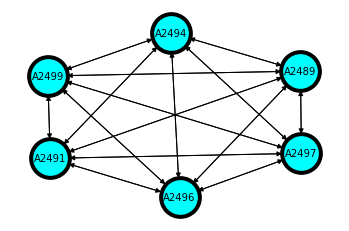
\includegraphics[scale=1]{graph.png}
\caption{One of the components with 6 nodes (Article IDs as node) }
\end{figure}

    \item \textbf{About human paths}\\
     \textbf{5} leaf Categories that are visited most in path finished by humans are namely \textbf{subject.Countries}, \textbf{subject.Geography.North-American-Geography},
    \textbf{subject.Geography.European-Geography.European-Countries}, \textbf{subject.Geography.Geography-of-Great-Britain},
    \textbf{subject.Science.Biology.General-Biology}.
    
    Whereas  \textbf{5} least visited leaf categories by human  namely \textbf{subject.Art.Artists}, \textbf{subject.History.Historians-chroniclers-and-history-books}, \textbf{subject.IT.Cryptography}, \textbf{subject.People.Producers-directors-and-media-figure},\textbf{subject.Citizenship.Conflict-and-Peace}.
    
\begin{figure}[H]
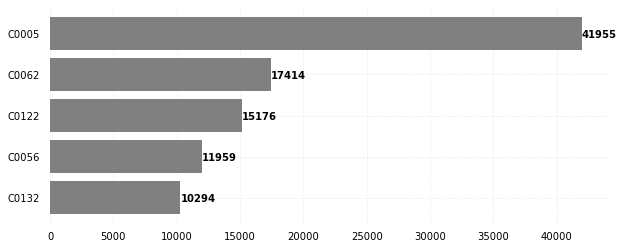
\includegraphics[scale=0.7]{bar1.png}
\caption{Showing 5 most visited categories(their ids on y-axis) with number of human paths visited them}
\end{figure}
    
    \item \textbf{About source and Destination:}\\
    \vspace{0.5cm}
    Total number of unique source and destination pairs obtained by from finished and unfinished human paths were \textbf{17196} out of which \textbf{10325} pairs where unique to finished human paths.\\
    \vspace{.5cm}
    Out of all \textbf{10325} source destination pairs obtained from finished human paths \textbf{91.6\%} were having average ratio of human path length to shortest path length between 1 and 2, \textbf{6.6\%} were having exactly 1, \textbf{1\%} between 2 and 3 and only \textbf{0.8\%} greater than 3. \
    
\begin{figure}[H]
\centering
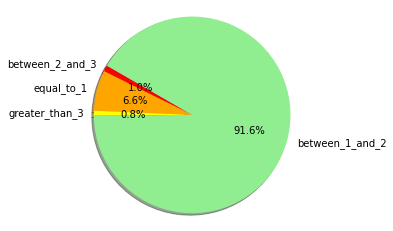
\includegraphics[scale=0.7]{pie.png}
\caption{Percentage of pairs having average ratio of human path length to shortest path length equal to 1, between 1 and 2,between 2 and 3 and greater than 3}
\end{figure}



 \end{enumerate}
 
\textbf{CONCLUSIONS}
\begin{enumerate}
    \item From the output of Question 7, \textbf{70.4\%} of the finished human paths were having length of human path greater than  the length of shortest path by just 2, and \textbf{82.5\%} finished human paths were having length of human path greater than the length of shortest path by just 3. Which signifies the fact that human intuitively tends to follow shortest paths without even knowing the actual shortest path among articles.
    
    \item From the pie chart above(Figure 3) , \textbf{98.2\%} of all source destination pairs in finished human paths were having average ratio of human path length to shortest path length less than equal to \textbf{2}. This shows that , when analysis is done on large number of source destination articles most of the time humans do follow the shortest path. 
    
\end{enumerate}
\end{document}